\documentclass[tikz,border=2pt]{standalone}
\usepackage{tikz}
\usetikzlibrary{arrows.meta,fit,positioning,shapes.geometric}
\definecolor{aegisblue}{HTML}{2F6DB3}
\definecolor{aegisgreen}{HTML}{3D8B6D}
\definecolor{aegisorange}{HTML}{D97732}
\definecolor{aegisgray}{HTML}{5B6470}
\begin{document}
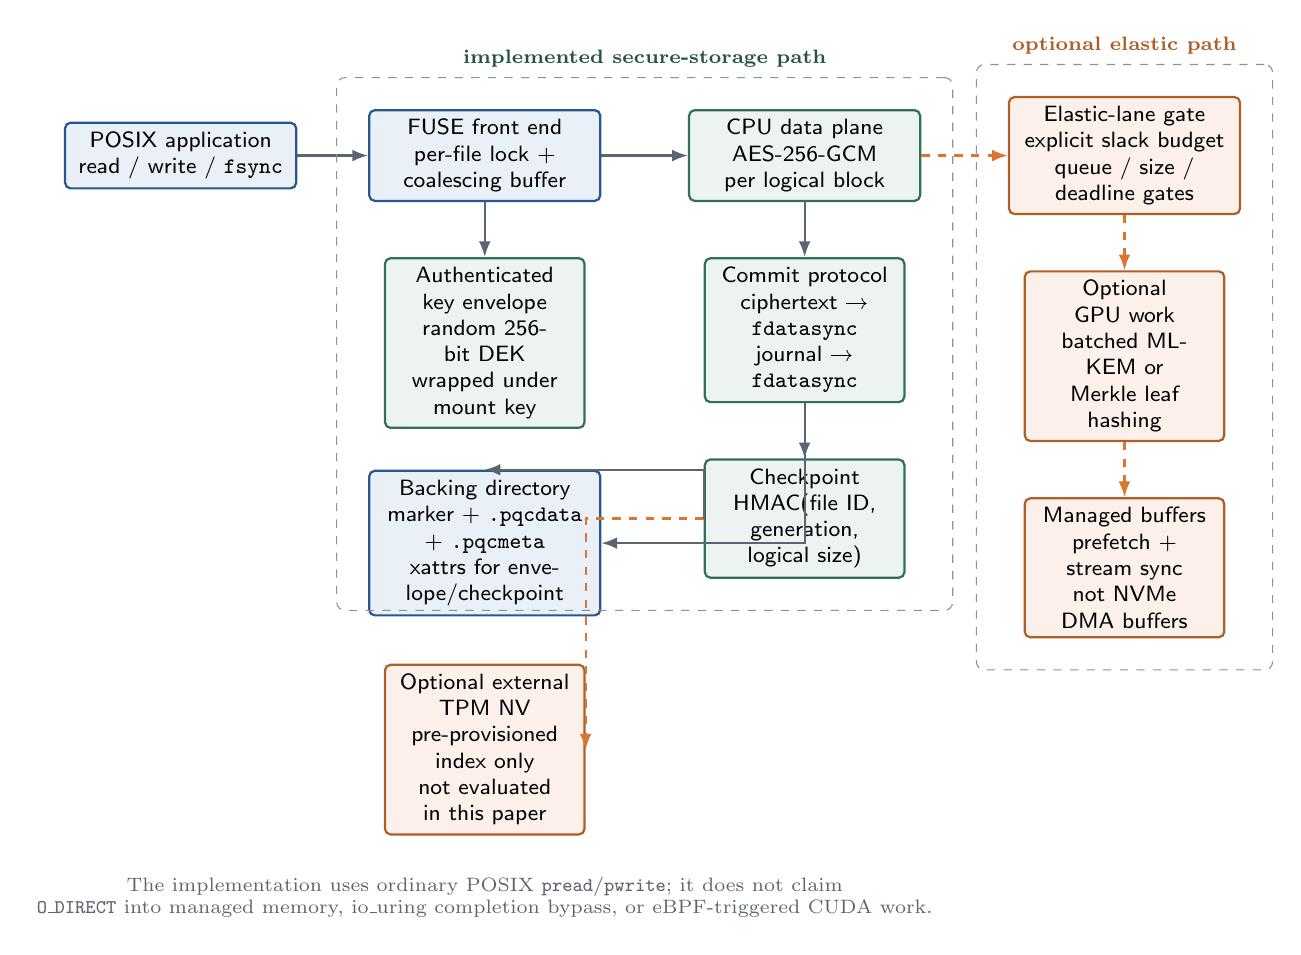
\begin{tikzpicture}[
  font=\sffamily\footnotesize,
  box/.style={rounded corners=2pt, draw=#1!80!black, fill=#1!10, thick,
              align=center, minimum height=8mm, text width=27mm},
  smallbox/.style={rounded corners=2pt, draw=#1!80!black, fill=#1!10, thick,
              align=center, minimum height=7mm, text width=23mm},
  plane/.style={rounded corners=3pt, draw=aegisgray!70, dashed, inner sep=4mm},
  flow/.style={-{Latex[length=2mm]}, thick, draw=aegisgray},
  opt/.style={-{Latex[length=2mm]}, thick, dashed, draw=aegisorange},
  note/.style={font=\scriptsize, align=center, text=aegisgray}
]
  \node[box=aegisblue] (app) {POSIX application\\read / write / \texttt{fsync}};
  \node[box=aegisblue, right=9mm of app] (fuse) {FUSE front end\\per-file lock +\\coalescing buffer};
  \node[smallbox=aegisgreen, below=7mm of fuse] (envelope) {Authenticated key envelope\\random 256-bit DEK\\wrapped under mount key};

  \node[box=aegisgreen, right=11mm of fuse] (cpu) {CPU data plane\\AES-256-GCM\\per logical block};
  \node[smallbox=aegisgreen, below=7mm of cpu] (journal) {Commit protocol\\ciphertext \textrightarrow{} \texttt{fdatasync}\\journal \textrightarrow{} \texttt{fdatasync}};
  \node[smallbox=aegisgreen, below=7mm of journal] (checkpoint) {Checkpoint\\HMAC(file ID, generation,\\logical size)};

  \node[box=aegisorange, right=11mm of cpu] (admission) {Elastic-lane gate\\explicit slack budget\\queue / size / deadline gates};
  \node[smallbox=aegisorange, below=7mm of admission] (gpu) {Optional GPU work\\batched ML-KEM or\\Merkle leaf hashing};
  \node[smallbox=aegisorange, below=7mm of gpu] (managed) {Managed buffers\\prefetch + stream sync\\not NVMe DMA buffers};

  \node[box=aegisblue, below=34mm of fuse] (store) {Backing directory\\marker + \texttt{.pqcdata} + \texttt{.pqcmeta}\\xattrs for envelope/checkpoint};
  \node[smallbox=aegisorange, below=6mm of store] (tpm) {Optional external TPM NV\\pre-provisioned index only\\not evaluated in this paper};

  \draw[flow] (app) -- (fuse);
  \draw[flow] (fuse) -- (cpu);
  \draw[flow] (fuse) -- (envelope);
  \draw[flow] (cpu) -- (journal);
  \draw[flow] (journal) -- (checkpoint);
  \draw[flow] (journal.south) |- (store.east);
  \draw[opt] (cpu.east) -- (admission.west);
  \draw[opt] (admission) -- (gpu);
  \draw[opt] (gpu) -- (managed);
  \draw[opt] (checkpoint.west) -| (tpm.east);
  \draw[flow] (checkpoint.west) |- (store.north);

  \node[plane, fit=(fuse)(envelope)(cpu)(journal)(checkpoint),
        label={[font=\scriptsize\bfseries,text=aegisgreen!60!black]above:implemented secure-storage path}] {};
  \node[plane, fit=(admission)(gpu)(managed),
        label={[font=\scriptsize\bfseries,text=aegisorange!80!black]above:optional elastic path}] {};
  \node[note, below=4mm of tpm] {The implementation uses ordinary POSIX \texttt{pread}/\texttt{pwrite}; it does not claim\\\texttt{O\_DIRECT} into managed memory, io\_uring completion bypass, or eBPF-triggered CUDA work.};
\end{tikzpicture}
\end{document}
